\chapter{Fractures}

We want to study the behaviour of water trapped in nanoscale (pores and) fractures in silica, so need want a way to generate and characterize such a structure. (Several methods of characterizing a fracture could be imagined (\hl{SOURCES, examples}), and we will use several of them.)        

\hl{terrain == heightmap??, finn bra ord her}

\section{Characterization}

\todo{change wording? copied from Fractals...}
An \emph{affine transformation} transforms a point $\bvec x = (x_1, \dots, x_n)$ into new points $\bvec x' = (r_1x_1, \dots, r_n, x_n)$, where the scaling rations $r_1, \dots, r_n$ are \emph{not} all equal.

A bounded set $\mathcal{S}$ is \emph{self-affine} if $\mathcal{S}$ is the union of $N$ non-overlapping subsets $\mathcal{S}_1, \dots, \mathcal{S}_N$, each of which is congruent to the set $\bvec r(\mathcal{S})$ obtained from $\mathcal S$ by the affine transform defined by $\bvec r$. Here \emph{congruent} means that the set of points $\mathcal{S}$ is identical to the set of points $\bvec r(\mathcal{S})$ after possible translations and/or rotations of the set\cite{feder1988fractals}.

A set $\mathcal{S}$ is \emph{statistically self-affine} if $\mathcal{S}$ is the union of $N$ non-overlapping subsets each of which is scaled down by $\bvec r$ from the original, and is identical in all statistical respects to $\bvec r(\mathcal{S})$.

\subsection{Hurst exponent}
\orangebox{
\begin{itemize}
    \item define fractal dimension
\end{itemize}
}

To characterize a fractal one can use the Hurst exponent, usually called $H$\footnote{\todo[inline]{The name used by Hurst in his work where he first describes the exponent was actually $K$\cite{hurst1965longterm}\cite{hurst1951longterm}}}, which comes from a statistical method developed by Hurst\cite{hurst1965longterm}\cite{hurst1951longterm}. The Hurst exponent is related to the fractal dimension $D$ by
\begin{align*}
    D = d-H,
\end{align*}
where $d$ is the spatial dimension of the fractal's domain\cite{feder1988fractals}.

The statistical method developed by Hurst is called \emph{rescaled range analysis} and was designed for use on 1-dimensional time series $f(t)$. The method has been generalized to higher dimensions\cite{fan2013rescaled}, but the original 1D form is shown here.

\subsubsection{Rescaled range analysis}
First the time series is divided into \todo{overlapping/non-overlapping?} intervals of length $\tau$. The average over each interval of length $\tau$ is
\begin{align*}
    \langle f \rangle_\tau = \frac{1}{\tau} \sum_{t=1}^\tau f(t).
\end{align*}
We let $F$ be the accumulated deviation from the mean
\begin{align*}
    F(t, \tau) = \sum_{t' = 1}^t \big( f(t') - \langle f \rangle_\tau \big).
\end{align*}
The difference between the maximum and minimum of the accumulated deviation from the mean is the \emph{range} R
\begin{align*}
    R(\tau) = \max_{1 \leq t \leq \tau} \big(F(t,\tau)\big) - \min_{1 \leq t \leq \tau} \big(F(t, \tau)\big).
\end{align*}
The standard deviation $S$ of the time series is estimated using
\begin{align*}
    S^2 = \frac{1}{\tau} \sum_{t=1}^\tau \big( f(t) - \langle f \rangle_\tau \big)^2.
\end{align*}
Hurst found that the observed \emph{rescaled range}, $R/S$, for many time series is described by the empirical relation\cite{feder1988fractals}
\begin{align*}
    \frac{R}{S} = \left(\frac{\tau}{2}\right)^H \sim \tau^H.
\end{align*}
We now see that we can estimate the Hurst exponent by a linear fit of the form
\begin{align*}
    \log \left(\frac{R}{S}\right) \sim H\log\tau,
\end{align*}
where we find $H$ as the slope of the linear fit.

\todo[inline]{Something about that it's hard to measure, and why.}

\subsubsection{Detrending moving average}
To estimate the Hurst exponent of a surface we use a method called detrending moving average (DMA) first described by E. Alessio, A. Carbone et al.\cite{alessio2002dma}, and later generalized to higher dimensions by A. Carbone \cite{carbone2007algorithm}. We use this method because ??? \todo[inline]{good results, easy to implement? }

We define a self-affine surface as $f(i,j)$, where $f$ is the height in the point $(i,j)$, defined in a discrete 2-dimensional domain with size $N\times N$, and with $i,j = 1,\dots,N$. We divide the surface into square \hl{subsurfaces} of size $n \times n$, and find the average $\tilde f_n$ of each subsurface by\footnote{\cref{eq:carbone_average} is how the average $\tilde f_n$ is stated in the article\cite{carbone2007algorithm}, but we rewrite it to \cref{eq:carbone_average_rewritten} so it's easier to understand. The two forms are equivalent.}
\begin{align}
    \tilde f_n(i,j) 
    &= \frac{1}{n^2}\sum_{k=-m}^{n-1-m} ~ \sum_{l=-m}^{n-1-m} f(i-k, j-l) \label{eq:carbone_average}\\
%     &= \frac{1}{n^2}\sum_{k=i-m}^{i-n+1+m}\sum_{l=j-m}^{j-n+1+m} f(i-k, j-l) \\
    &= \frac{1}{n^2} \sum_{k=(i+m)-n+1}^{i+m} ~ \sum_{l=(i+m)-n+1}^{i+m} f(k, l), \label{eq:carbone_average_rewritten}
\end{align}
where
\begin{align*}
    &m = \left \lfloor n\theta \right \rfloor &\text{for }0 \leq \theta < 1,
\end{align*}
which means that $0 \leq m \leq (n-1)$. $\theta$ is a parameter that controls the position of the square relative to the point $(i,j)$. There are three notable cases for $\theta$, which are listed below, and are illustrated in \cref{fig:DMA_theta}.
\begin{itemize}
    \item For $\theta = 0$ we have $m=0$ and we average over a square with the point $(i,j)$ in the square's upper right corner (($i-n+1) \leq k,l \leq i$). See \cref{fig:DMA_theta_a}.
    \item For $\theta = 1/2$ we average over a square centered on the point $(i,j)$. See \cref{fig:DMA_theta_b}.
    \item For $\theta = (n-1)/n$ we have the maximum value for $m$, $m=n-1$, and average over a square with the point $(i,j)$ in the square's lower left corner \todo{THESE LIMITS ARE WRONG??}($i \leq k,l \leq (i+n-1)$). See \cref{fig:DMA_theta_c}.
\end{itemize}

\begin{figure}
    \centering
    \begin{subfigure}[b]{0.25\textwidth}
        \includesvg[width=\textwidth, svgpath=./images/Hurst/]{2DDMA_theta04_a}
%         \caption{Illustration of how to divide a convex hexahedron into five tetraheda.}
        \caption{$\theta = 0$}
        \label{fig:DMA_theta_a}
    \end{subfigure}
    \hspace{0.1\textwidth}
    \begin{subfigure}[b]{0.25\textwidth}
        \includesvg[width=\textwidth, svgpath=./images/Hurst/]{2DDMA_theta04_b}
%         \caption{A random fracture made from two periodic heightmaps.}
        \caption{$\theta = 1/2$}
        \label{fig:DMA_theta_b}
    \end{subfigure}
    \hspace{0.1\textwidth}
    \begin{subfigure}[b]{0.25\textwidth}
        \includesvg[width=\textwidth, svgpath=./images/Hurst/]{2DDMA_theta04_c}
%         \caption{A random fracture made from two periodic heightmaps.}
%         \caption{$\theta \rightarrow 1$ \\ ($\theta = (n-1)/n$)}
%         \caption{$\theta \rightarrow 1$}
        \caption{$\theta = (n-1)/n$}
        \label{fig:DMA_theta_c}
    \end{subfigure}
        \caption{
        Illustration of what the parameter $\theta$ controls in the detrending moving average method in 2 dimensions. The circles are points where the surface is defined, the red star is the point $(i,j)$, and the black square encompasses the points averaged over to calculate $\tilde f_n(i,j)$ in \cref{eq:carbone_average_rewritten}. The illustration uses $n = 3$.
        \label{fig:DMA_theta}
    }
\end{figure}

We then define the generalized variance $\sigma_\text{DMA}^2$
\begin{align*}
    \sigma_\text{DMA}^2 
    = \frac{1}{(N-n)^2}\sum_{i=n-m}^{N-m} ~ \sum_{j=n-m}^{N-m} 
    \big(
        f(i,j) - \tilde f_n(i,j)
    \big)^2,
\end{align*}
where we see that $f(i,j) - f_n(i,j)$ is the difference between the point $(i,j)$ and the average of a square of points (including the point itself) of size $n \times n$, as explained above (see \cref{fig:DMA_theta}).
% (the position of the square is controlled by the parameter $\theta$, as explained above, and illustrated \cref{fig:DMA_theta}). 
The summation limits $(n-m) \leq i,j \leq N-m$ are set so that the averages $f_n(i,j)$ don't exceed the domain with size $N \times N$.

The generalized variance goes as
\begin{align*}
    \sigma_\text{DMA}^2 \sim \left(2n^2\right)^H,
\end{align*}
which we can use to find the Hurst exponent $H$, by calculating $\sigma_\text{DMA}^2$ for different sizes of the squares, $n$. We estimate $H$ by a linear fit of $\log \sigma_\text{DMA}^2$ against $\log 2n^2$, where $H$ is the slope.

In the paper that generalizes DMA to higher dimensions\cite{carbone2007algorithm} they use different parameters for each spatial dimension $d$, $\bvec\theta = \theta_1, \dots, \theta_d$ and $n_1, \dots, n_d$, but for simplicity and to avoid \hl{strange} results, we use $\theta_1 = \theta_2 = \theta$ and $n_1 = n_2 = n$.

% With $\theta = 0$ we have $m = 0$ and average over all points $(\leq k \leq i,l \leq j)$. 

% With $\theta = n/(n-1)$ we have $m = n-1$, and average over all points $(k \geq i,l \geq j)$.

% We define the generalized variance $\sigma_\text{DMA}^2$ as the variance 
% \begin{align*}
%     \sigma_\text{DMA}^2 
%     = \frac{1}{(N-n)^2}\sum_{i=n-m}^{N-m}\sum_{j=n-m}^{N-m} 
%     \big(
%         f(i,j) - \tilde f_n(i,j)
%     \big)^2,
% \end{align*}
% where\footnote{We rewrite \cref{eq:carbone_average} for easier understanding}
% \begin{align}
%     \tilde f_n(i,j) 
%     &= \frac{1}{n^2}\sum_{k=-m}^{n-1-m}\sum_{l=-m}^{n-1-m} f(i-k, j-l) \label{eq:carbone_average}\\
% %     &= \frac{1}{n^2}\sum_{k=i-m}^{i-n+1+m}\sum_{l=j-m}^{j-n+1+m} f(i-k, j-l) \\
%     &= \frac{1}{n^2} \sum_{k=(i+m)-n+1}^{i+m} ~ \sum_{l=(i+m)-n+1}^{i+m} f(k, l).\nonumber %\label{eq:carbone_average_rewritten}
% \end{align}
% \begin{align*}
%     m = \left \lfloor n\theta \right \rfloor
% \end{align*}
% $\theta = 1$ or $\theta = 0$ (directed implementation, for fractals with preferential growth direction) \\
% $\theta = 0.5$ (isotropic implementation, ``uniformity in all orientations'') \\



% \begin{figure}
%     \centering
%     \includesvg[width=0.99\textwidth, svgpath=./images/Hurst/]{2DDMA_theta04}
%     \caption{
%         Illustration of what the parameter $\theta$ controls in the detrending moving average method in 2 dimensions. The circles are points where a surface is defined, the red star marks the point $(i,j)$, and the black square marks the points averaged over to calculate $\tilde f_n(i,j)$ in \cref{eq:carbone_average_rewritten}.
%         \label{fig:DMA_theta}
%     }
% \end{figure}



% \subsubsection{Detrended fluctuation analysis in higher dimensions}
% original DFA\cite{peng1994mosaic}
% HDDMA\cite{gu2006detrended}
% 
% To estimate the Hurst exponent of a fracture we use a generalized version of a method called \emph{detrended fluctuation analysis}\cite{peng1994mosaic}, which was generalized to higher dimensions by Gu and Zhou\cite{gu2006detrended}.
% 
% The two-dimensional DFA:
% 
% We have a self-affine surface stored in the matrix $f(i,j)$, where $f$ \hl{is} the height of the surface in the point $(i,j)$, with $i,j = 1,\dots,N$, and $N^2$ is the number of points where the surface is defined. The surface is divided into $n\times n$ disjoint (non-overlapping) \hl{and neighboring} surfaces \todo{sub-surface?} of the same size $s\times s$, where $n = N/s$. Each of these surfaces is denoted by $f_{u,v}$ such that $f_{u,v}(i,j) = f(i+k, j+l)$ for $i,j = 1, \dots, s$, where $k = (u-1)s$ and $l = (v-1)s$.
% 
% For a surface $f_{u,v}$ the cumulative sum $F_{u,v}(i,j)$ is calculated as follows
% \begin{align*}
%     F_{u,v}(i,j) = \sum_{m=1}^i\sum_{n=1}^j f_{u,v}(m,n),
% \end{align*}
% where $i,j = 1,\dots,s$. Note that F_{u,v}(i,j) itself is a surface.
% 
% The trend of the constructed surface $F_{u,v}$ can be determined by fitting it with a polynomial $\tilde F$



\todo[inline]{implemented in Matlab/Octave}

\subsection{Surface area}
\subsection{Distance to nearest atom}
\begin{itemize}
    \item Fractals
    \item Fractional Brownian Motion
    \item The Hurst Exponent
\end{itemize}

\section{Generating fractures}
\hl{Stuff to define?}
\begin{itemize}
    \item fBm surfaces
    \item Hurst exponent
    \item Gaussian random variable ?
    \item non-stationary
    \item self-similar
    \item isotropic
    \item lacunarity
\end{itemize}

\subsection{Generating terrains}
% When generating random terrain we want to be able to control the properties like the Hurst exponent (\hl{etc.?}) of the terrain.

To generate our random terrains we use an iterative midpoint displacement method usually called successive random additions \hl{(SRA)}. The method is based on a method proposed by Fourner in 1982\cite{fournier1982computer}, but with some modifications suggested by Voss\cite{voss1985random, voss1988fractals}. The method has further been discussed by Saupe\cite{saupe1988algorithms}, amongst others. We choose this method mainly because it's possible to generate periodic terrains with it, because it generates very good approximations to fBm surfaces\cite{zhou2005comparison}, and because the Hurst exponent of the generated terrains is easy to control. The method is also easy to understand, easy to implement, and generates terrains with high resolution very fast. The method is widely used in scientific applications\hl{cite??} because of these properties, and is also used for generating terrains in computer graphics, since the terrains look very realistic \hl{with only some minor artefacts?? (high, narrow peaks)}.

The method is very similar to the standard midpoint displacement method, which in 1 dimension goes as follows. See \cref{fig:midpoint01} for a visual presentation.
\begin{enumerate}
    \item Give the values at the endpoints $y_0$ and $y_n$ random values from a Gaussian random variable with mean $\mu = 0$ and variance $\sigma_0^2$. The variance can be chosen freely.
    \item Generate the value in the center of the interval, $y_{n/2}$, by averaging the two endpoints and adding a Gaussian random number with mean $\mu = 0$ and variance
    \begin{align*}
         \sigma_1^2 = \left(1/2\right)^{2H}\sigma_0^2,
    \end{align*}
    where $H$ is the wanted Hurst exponent.
    \item Continue generating the values in the center of each interval until you reach the desired number of points, while reducing the variance of the random number by a factor $\frac{1}{2}$ each iteration. For iteration $i$ we have
    \begin{align*}
        \sigma_i^2 = \left(1/2\right)^{i2H}\sigma_0^2.
    \end{align*}
\end{enumerate}
This method generates a \hl{1-dimensional line}, with a Hurst exponent close to the input $H$. But since we only add random numbers to the new values, the result is non-stationary for $H \neq 0.5$\cite{voss1985random}\hl{, and it is neither self-similar or isotropic, as noted by Mandelbrot}\cite{mandelbrot1982comment}. To mitigate this we implement the addition suggested by Voss\cite{voss1985random}, which consists of adding a random number to all points in each iteration. Voss called this modified method ``successive random additions''.

\begin{figure}
    \centering
    \includesvg[width=0.5\textwidth, svgpath=./images/diamond_square/]{random_midpoint_displacement_regular02}
    \caption{
        Caption.
        \label{fig:midpoint01}
    }
\end{figure}

% \begin{figure}
%     \centering
%     \includesvg[width=0.7\textwidth]{images/test/diamondSquare02}
%     \caption{
%         \hl{TEST}
%     }
% \end{figure}

Voss has geneneralized the the method of SRA to higher dimensions\cite{voss1985random}, which is the algorithm we will be using. We will generate heightmaps, meaning a 2-dimensional grid of points ($x_i$, $y_i$), with a value for the height in each point ($z_i$) which is generated by the algorithm.

% \hl{Now, generating fBm in one dimension is all well and good}, but we need to generate a 2/3 dimensional terrain. For simplicity we generate a \emph{heightmap}, meaning a 2-dimensional grid of points ($x_i$, $y_i$), with a value for the height in each point ($z_i$) which is generated by the algorithm. Luckily, Voss has generalized the successive random additions algorithm to higher dimensions, which is what we will be using.

\hl{To explain the algorithm} we start with a simple case of an infinite grid of evenly spaced points, all with known $z$-values. This allows us to first focus on the central part of the algorithm which consists of two steps; often called the ``diamond step'' and the ``square step''. We take on a set of 2x2 points in the grid, as seen in the leftmost square of \cref{fig:initial_square_step}.
\begin{enumerate}
    \item \emph{The square step}: We have four points that make up a square. The $z$-value in the center of the square is generated by averaging the $z$-values of the four corners of the square, as indicated by the red dots in \cref{fig:initial_square_step}, and adding a random Gaussian number with mean $\mu = 0$ and variance $\sigma_0^2$ to both the new point and the old points. The variance can be chosen freely.
    \label{enum:test}
    
    \item \emph{The diamond step}: The $z$-values in the middle of the four edges of the square is generated by averaging the $z$-values of the points above, below, to the right of, and to the left of the points, as indicated by the red dots in \cref{fig:diamond_step}, and adding a random Gaussian number with mean $\mu = 0$ and a \emph{reduced} variance $\sigma_1^2 = \sigma_0^2r^{2H}$, where $H$ is the wanted Hurst exponent, and $r < 1$ is a parameter that controls the \hl{\emph{lacunarity} of the fractal}, to all new and old points.
    
%     \item We now see that we can apply the square step four times on the resulting grid (see the rightmost square in \cref{fig:diamond_step}), as illustrated in \cref{fig:square_step}, and then keep increasing the resolution by alternating between the two methods.
%     
%     For step $i$ of the algorithm the variance of the Gaussan variable is
%     \begin{equation}
%         \sigma_i^2 = \sigma_0^2\left(r^n\right)^{2H},
%     \end{equation}
%     where $\sigma_0^2$ is the initial variance.
    
%     \item \emph{The square step}: These nine points make up four squares. We generate the $z$-values in the center of each square by averaging the $z$-values of the four corners in each square, indicated by the red dots in \cref{fig:square_step}, and adding a random Gaussian number with mean $\mu = 0$ and variance $\sigma_0$.
    
%     \item \emph{The diamond step}: We now zoom in on the five points in the corner of the rightmost square in \cref{fig:square_step}, making up a square with a point in the center, as seen in the leftmost square in \cref{fig:diamond_step}. We now generate the $z$-values in the center of each edge of this square by averaging the $z$-values of the four corners of a diamond, made up by the three points in our view, and one point outside of our zoomed in view \hl{(since we have an infinite grid, this shouldn't cause any problems)}, indicated by the red dots in \cref{fig:diamond_step}.
\end{enumerate}

We now see that we can apply the square step four times on the resulting grid (see the rightmost square in \cref{fig:diamond_step}), as illustrated in \cref{fig:square_step}, and then keep increasing the resolution by alternating between the two methods. For step $i$ of the algorithm the variance of the Gaussan variable becomes
\begin{equation}
    \sigma_i^2 = \sigma_0^2\left(r^n\right)^{2H},
\end{equation}
where $\sigma_0^2$ is the initial variance.

\hl{Since we add a random number to all points in each step of this algorithm, we can change the variance of the random number with any factor $r<1$ each step.}

% The algorithm can be seen in \cref{fig:diamond_square}.
% 
% \begin{enumerate}
%     \item \hl{(Initial steps)} The $z$-values in the four corners ($x_0$, $y_0$), ($x_0$, $y_n$), ($x_n$, $y_0$) and ($x_n$, $y_n$), is drawn from a Gaussian distribution with mean $\mu = 0$ and variance $\sigma_0^2$.
%     \item \hl{(Initial steps)} The $z$-value in the center ($x_{n/2}$, $y_{n/2}$) is calculated as the average of the four corners, plus a Gaussian random number with variance $\sigma_1 = $
%     \item \hl{(Diamond step)} The $z$-values in the center of the four edges is calculated as the average
% \end{enumerate}
% 
% Since we're using periodic boundary conditions in our simulations, we need the terrains to be periodic as well, which means that we have to take special care to what happens near the edges when generating them. 

\begin{figure}
    \centering
    
    \setlength{\myfigwidth}{0.9\textwidth}
    \setlength{\mycaptionwidth}{0.09\textwidth}
    

    \begin{minipage}[c]{\myfigwidth}
        \includesvg[width=\textwidth, svgpath = images/diamond_square/]{initial_square_step_leftaligned}
    \end{minipage}
    \begin{minipage}[c]{\mycaptionwidth}
%         \captionsetup{singlelinecheck=false,width=\textwidth}
%         \captionsetup{width=\textwidth}
%         \subcaption{90 degrees (vertical), 579 min.}
        \subcaption{}
        \label{fig:initial_square_step}
    \end{minipage}
    \\ \smallskip
    
    \begin{minipage}[c]{\myfigwidth}
        \includesvg[width=\textwidth, svgpath = images/diamond_square/]{diamond_step}
    \end{minipage}
    \begin{minipage}[c]{\mycaptionwidth}
%         \captionsetup{singlelinecheck=false,width=\textwidth}
%         \captionsetup{width=\textwidth}
%         \subcaption{90 degrees (vertical), 579 min.}
        \subcaption{}
        \label{fig:diamond_step}
    \end{minipage}
    \\ \smallskip
    
    \begin{minipage}[c]{\myfigwidth}
        \includesvg[width=\textwidth, svgpath = images/diamond_square/]{square_step}
    \end{minipage}
    \begin{minipage}[c]{\mycaptionwidth}
%         \captionsetup{singlelinecheck=false,width=\textwidth}
%         \captionsetup{width=\textwidth}
%         \subcaption{90 degrees (vertical), 579 min.}
        \subcaption{}
        \label{fig:square_step}
    \end{minipage}
    
    
%     \begin{minipage}[c]{\myfigwidth}
%     \begin{subfigure}[b]{0.9\textwidth}
% %         \includesvg[width=0.9\textwidth]{images/diamond_step}
%         \includesvg{images/diamond_step}
%         \caption{A gull}
%         \label{fig:gull}
%     \end{subfigure}
%     \\
%     \begin{subfigure}[b]{0.9\textwidth}
% %         \includesvg[width=0.9\textwidth]{images/square_step}
%         \includesvg{images/square_step}
%         \caption{A gull}
%         \label{fig:gull2}
%     \end{subfigure}

    \caption{
        New points are black, old points are grey, and points used in the generation of the new points are red.
        \label{fig:diamond_square}
    }
\end{figure}


We obviously can't generate infinite terrains, so some special cases need to be addressed near the boundaries of the terrain. We also want the generated terrains to be periodic, meaning that they should behave nicely when repeated in the $x$- and $y$-direction. This leaves us with the following final algorithm
\begin{enumerate}
    \item Start with a set of four points, located in the corners of a grid. These points all need to have the same $z$-value, since the final terrain must be periodic.
    \item Generate the $z$-value in the center of the grid using the square step, by averaging over the four neighbors, as shown in \cref{fig:initial_square_step}. Add a random Gaussian number with mean $\mu = 0$ and variance $\sigma^2 = \sigma_0^2$ to the new point, and to the point in the top left corner. Set the three other corners equal to the top left corner, to keep the terrain periodic.
    \item Generate the values in the middle of the top and left edge of the grid using the diamond step from before. Add a random Gaussian number with mean $\mu = 0$ and variance $\sigma_1^2 = \sigma_0^2r^{2H}$, where $H$ is the wanted Hurst exponent. Since the terrain is periodic, we can wrap around the edges to reach the points beyond the edges of our grid (the points outside the grid in \cref{fig:diamond_step}). Set values in the middle of the right and bottom edge equal to the corresponding values in the middle of the left and top edge, to keep the terrain periodic\footnote{\hl{We could have done this in a slightly different way, by making the grid one unit smaller, and starting with only one point in one of the corners, but by doing it the way we have we can keep the square step the same as before.}}.
    
%     \item We now need to generate the $z$-values in the middle of the four edges of the grid, using the diamond step. But since we have a finite and periodic grid, we have to wrap around the edges when taking the average over the four neighbours. We also see that the top and bottom edge, and the left and right edge should be equal after generating the new points\footnote{\hl{We could have done this in a slightly different way, by making the grid one unit smaller, and starting with only one point in one of the corners, but doing it the way we have we can keep the square step the same as before.}}, to keep the grid periodic. This can for example be done by generating the point in the middle of the left edge and the point in the middle of the top edge by using the diamond step and wrapping around the edges, and then setting the corresponding points on the right and bottom edge equal to the generated points.
    
%     This can for example be done by only generating the points on the top and left edge, and then setting the points on the right edge equal to the left edge, and the points on the .

    \item Continue generating new points and increasing the resolution of the \hl{terrain/grid} until you reach the desired number of \hl{points/resolution}. We see in \cref{fig:square_step} that the square step doesn't need any changes, since we don't generate any points at the edges of the grid, and we never have any neighbors that are beyond the edges of the grid. For the diamond step we need to make sure we wrap around the edges to find neighbors when calculating points that are close to the edges of the grid, and that we update the left and bottom edges as needed. 
    
    For step $i$ the variance of the random Gaussian number is
    \begin{align*}
        \sigma_i^2 = \sigma_0^2(r^i)^{2H}.
    \end{align*}
\end{enumerate}

See \cref{fig:diamond_square_terrain} for a terrain generated by the algorithm.

\begin{figure}
    \centering
    \includesvg[width=0.7\textwidth, svgpath=./images/diamond_square/surface_example/]{surface_labels}
    \caption{
        Caption.
        \label{fig:diamond_square_terrain}
    }
\end{figure}

\orangebox{
{\bf Notes:}
\begin{itemize}
    \item Size of surface $(2^n+1)$
    \item Edges / bottom/top edge
\end{itemize}

{\bf Stuff:}
\begin{itemize}
    \item Diamond-square -- why and how
    \item Periodic/non-periodic
    \item Lacunarity
\end{itemize}
Implementation (in Matlab/C++)?
}

% \begin{figure}
%     \centering
%     \def\svgwidth{\textwidth}
%     \input{images/diamondSquare02.eps_tex}
% \end{figure}

% \begin{figure}
%     \centering
%     \def\svgwidth{\textwidth}
%     \input{images/diamondSquare03.pdf_tex}
% \end{figure}

% \subsection{Successive Random Addition}
% To generate a random heightmap with a known Hurst exponent we used the successive random addition (SRA) algorithm introduced by Voss\cite{voss1985random}. It is a variation of a simpler algorithm called random midpoint displacement (RMD), a subdivision method described by, amongst others, Fournier, Fussell, and Carpenter\cite{fournier1982computer, carpenter1980computer}. To illustrate how the algorithms work, we will start with a simple 1-dimensional example of RMD.
% 
% We start with two points $Y(0)$ and $Y(1)$ at the edges of our interval. We find a point $Y(\frac{1}{2})$ in the center of the interval by interpolating the two initial points, and adding a Gaussian random number with zero mean and variance $\sigma^2$
% 
% \subsection{Midpoint Displacement Method}
% The most basic method we used is a very basic but widely used method, which has many variations and names. The most common names are ``the diamond-square algorithm''\hl{cite}, ``the midpoint displacement method''\hl{cite}, ``plasma fractal'' and ``cloud fractal''.
% 

\subsection{Generating fractures from terrains}
To generate a realistic fracture we use the method of successive random additions, as described previously, to generate random heightmaps with a known Hurst exponent. If we generate two of these terrains we can make a fracture by putting one terrain above the other, and letting either the space between or outside the heightmaps be the void. Since we are using periodic systems the two different approaches are equivalent, but we chose to let the space between the heightmaps be the void, for easier visualization.

In practice we make a fracture using the following procedure
\begin{itemize}
    \item Generate two heightmaps.
    \item Rescale the $x$- and $y$-positions of all points in the heightmaps, so they span the size of the atomic system.
    \item Rescale the $z$-values of the heightmaps so all points are inside the system.
    \item Remove all atoms between the upper and lower heightmap.
\end{itemize}

Removing all atoms between the two heightmaps isn't a trivial task. We do this by utilizing the fact that the points in each heighmap lie on a regular grid in the $x$-$y$-plane, to divide the volume into tetrahedra. If the two heightmaps are not intersecting, we see that we can divide the volume between them into convex hexahedra, one for each set of points
($x_{i}, y_{i}$), ($x_{i}, y_{i+1}$), ($x_{i+1}, y_{i}$), and ($x_{i+1}, y_{i+1}$) 
% $(x_i, y_i)$  $(x_i, y_{i+1})$ $(x_{i+1}, y_i)$ $(x_{i+1}, y_{i+1})$
in the $x$-$y$-grid. Each of these hexahedra can then be divided into five tetrahedra, as illustrated in \cref{fig:hex_to_tetra}.

% \begin{figure}
%     \centering
%     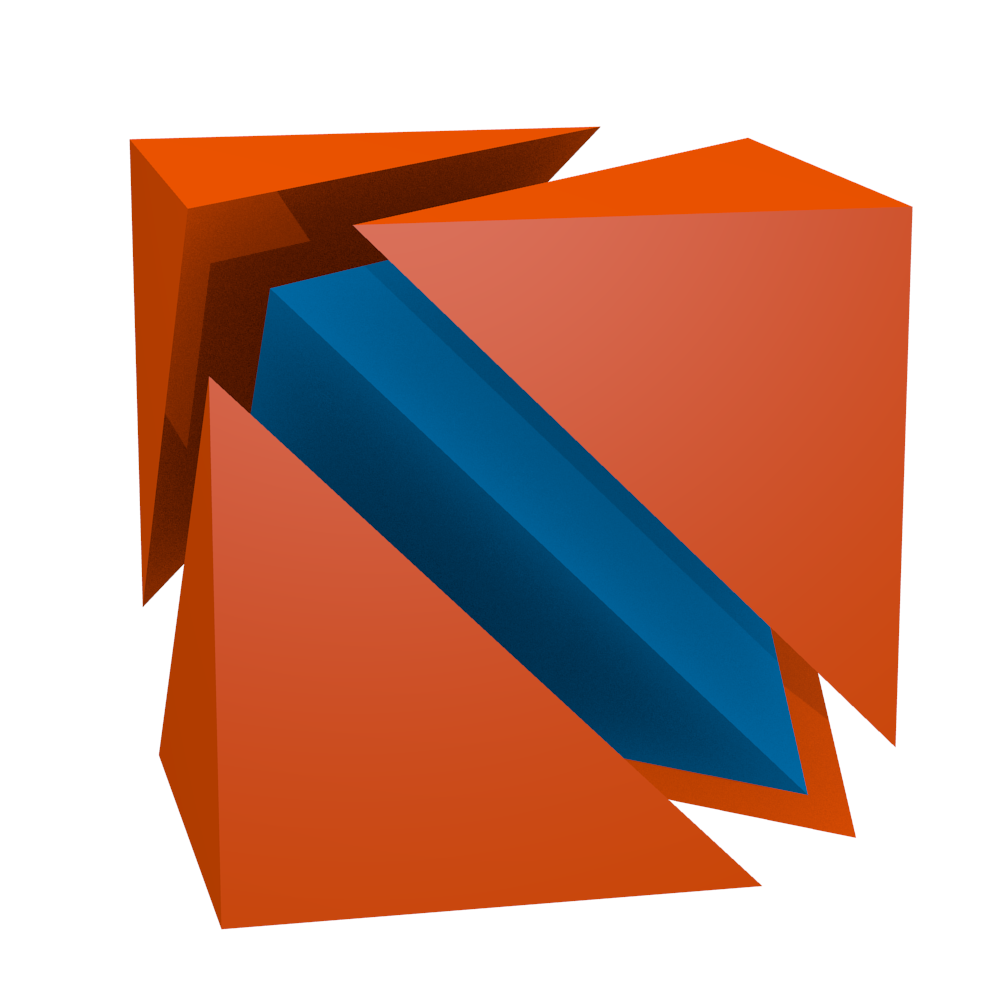
\includegraphics[width=0.4\textwidth]{images/fracture/hexahedron_to_tetrahedra.png}
%     \caption{
%         Illustration of how to divide a hexahedron into five tetraheda.
%         \label{fig:hex_to_tetra}
%     }
% \end{figure}
% 
% \begin{figure}
%     \centering
%     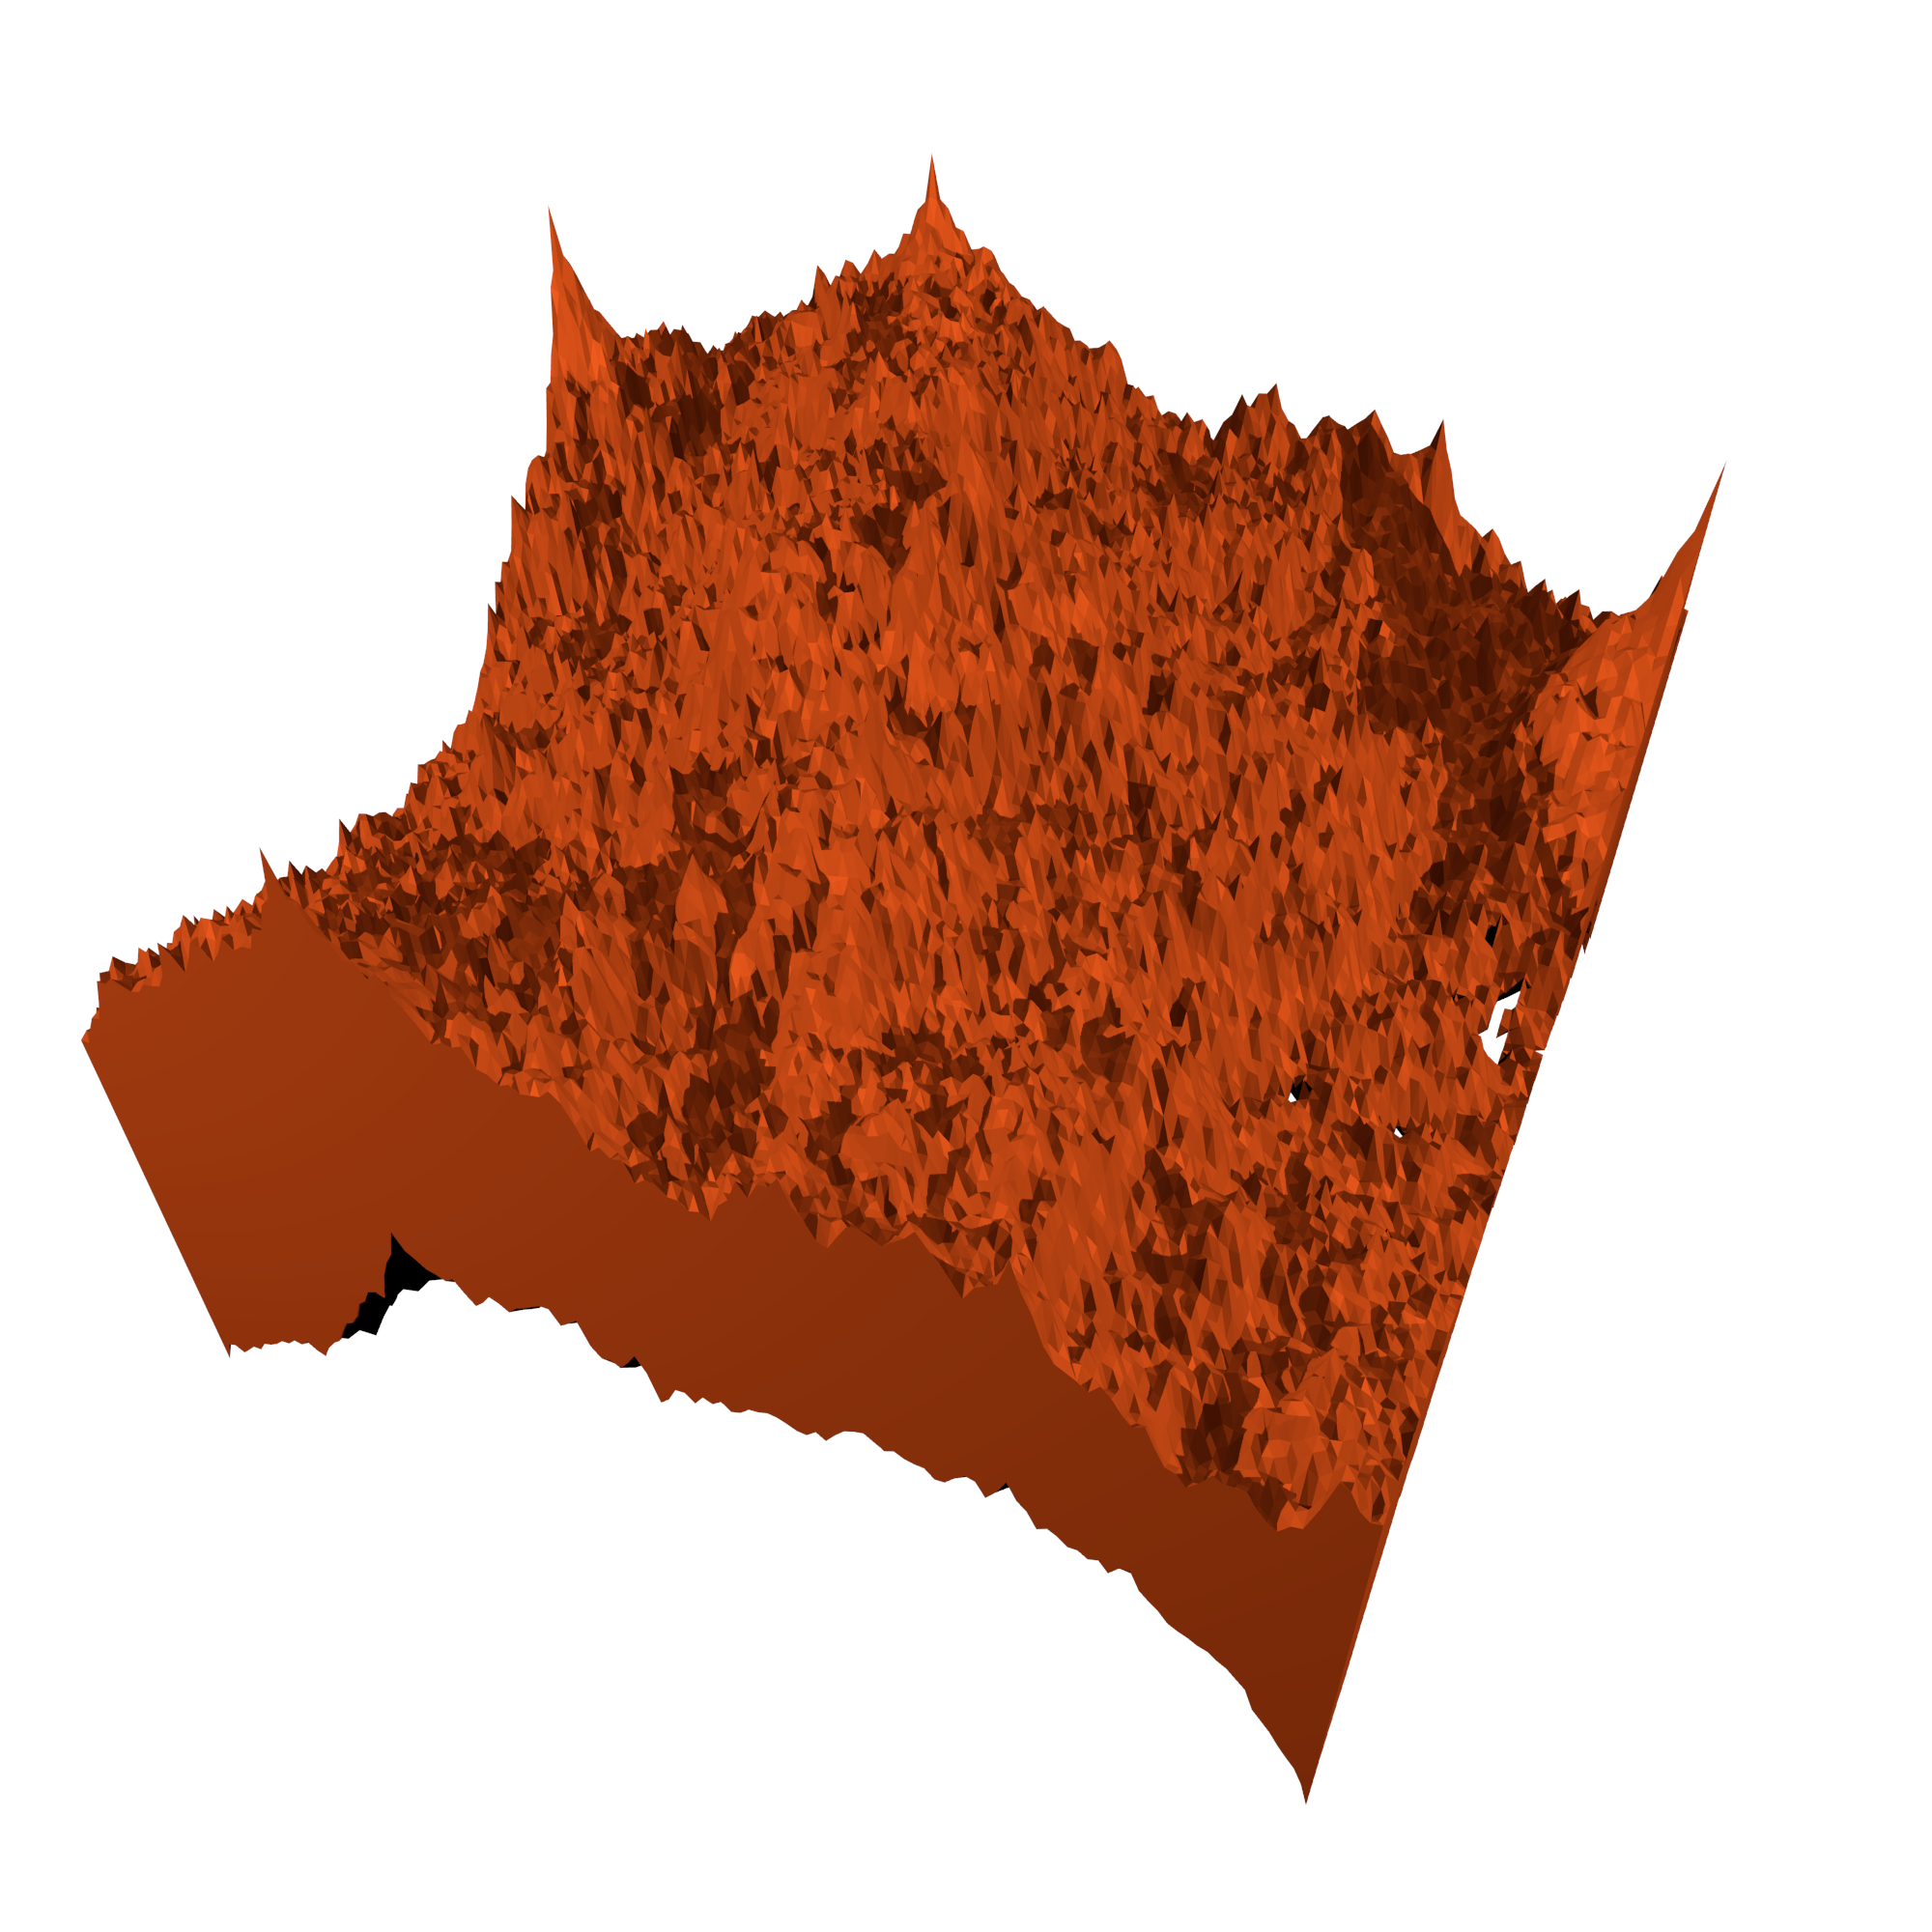
\includegraphics[width=0.6\textwidth]{images/fracture/fracture.png}
%     \caption{
%         A model of a fracture.
%         \label{fig:fracture_model}
%     }
% \end{figure}

\begin{figure}
    \centering
    \begin{subfigure}[b]{0.35\textwidth}
        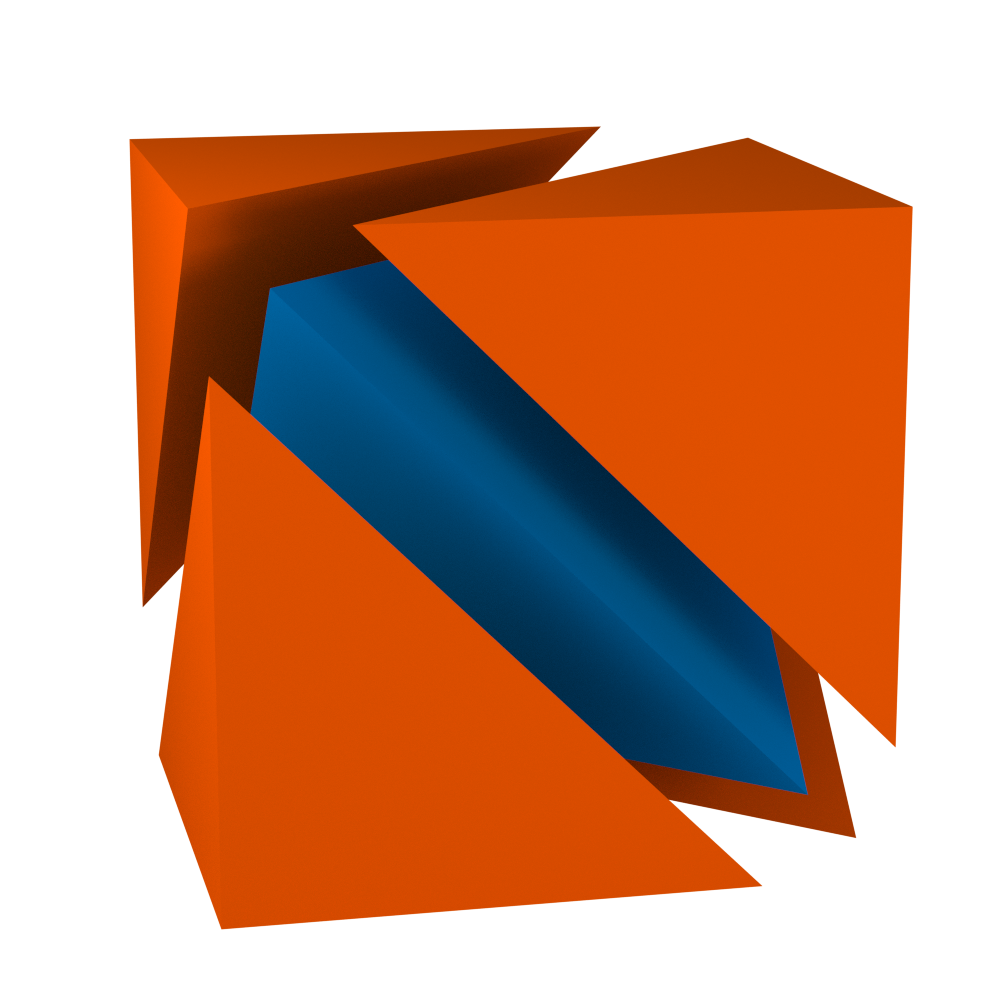
\includegraphics[width=\textwidth]{images/fracture/hexahedron_to_tetrahedra01_cycles_n200.png}
        \caption{Illustration of how to divide a convex hexahedron into five tetraheda.}
        \label{fig:hex_to_tetra}
    \end{subfigure}
    \hspace{5mm}
    \begin{subfigure}[b]{0.55\textwidth}
        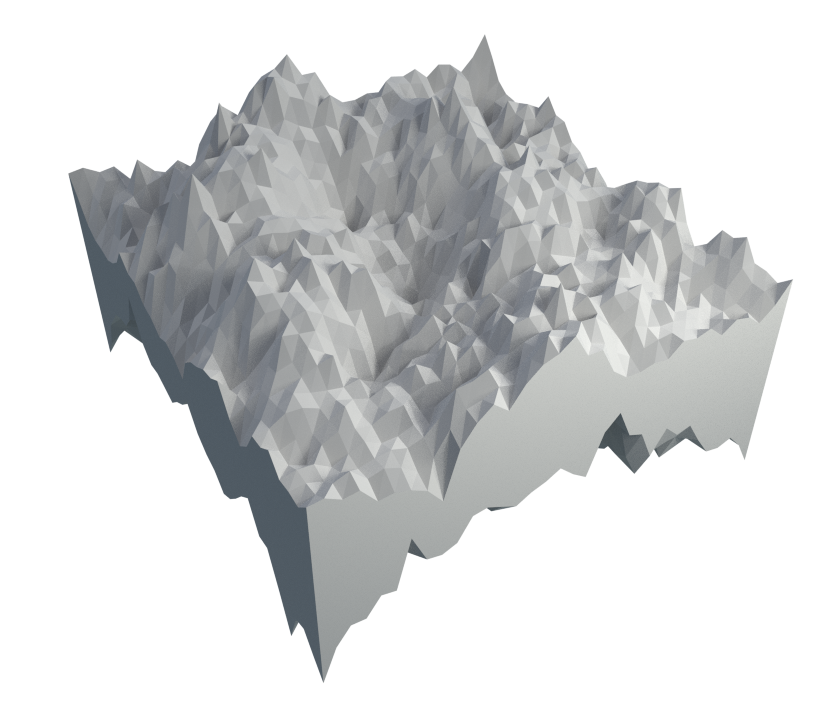
\includegraphics[width=\textwidth]{images/fracture/fracture05_n200.png}
        \caption{A random fracture made from two periodic heightmaps.}
        \label{fig:fracture_model}
    \end{subfigure}
\end{figure}

\subsubsection{Finding a point inside a tetrahedron}
% To calculate if a point is inside a tetrahedron we utilize the \emph{oriented} volume of a tetrahedron. The oriented volume of a tetrahedron with vertices $\bvec a$, $\bvec b$, $\bvec c$ and $\bvec d$ can be calculated as
% \begin{align*}
%     V = \frac{1}{6}(\bvec a - \bvec d)\big[(\bvec b - \bvec d)\times(\bvec c - \bvec d)\big].
% \end{align*}
% The \emph{ordered} volume simply means that the order of the vertices will determine the sign of the volume. The sign of the volume will be determined by on which side of the plane between $\bvec b$, $\bvec c$ and $\bvec d$ the point $\bvec a$ lies. The cross product $(\bvec b - \bvec d)\times(\bvec c - \bvec d)$ gives a normal vector to the plane, and the dot product projects $(\bvec a - \bvec d)$ onto this normal. The sign of the dot product is positive if $\bvec a$ is located the side of the plane which the normal points towards, and negative else.

% We then compare the sign of the volume of the tetrahedra to the signs of the volumes of four tetrahedra constructed by replacing one of the vertices of the tetrahedra with the point we want to find out if is inside the tetrahedra.



% A tetrahedron consists of four points 
% % $\bvec a$, $\bvec b$, $\bvec c$, and $\bvec d$, 
% % $\bvec r_i$ for $i\in\{1,2,3,4\}$,
% % $x$, $b$, $c$, and $d$, 
% $x_i$ for $i\in\{1,2,3,4\}$,
% and four faces spanned out by the four possible combinations of the four points. For a face spanned by the vectors $\bvec r_i = x_i - x_j$ and $\bvec r_j = x_k - x_j$, where, we can see if a point $P$ is on the same side of the face as the point $\bvec x_{l\neq i,j,k}$ not used to construct the face by doing some geometry. We calculate the normal vector to the face by the cross product $\bvec n = \bvec r_i\times\bvec r_j$. This gives us a normal vector $\bvec n$ to the surface. We then find the sign of dot products $\bvec n (P - x_j)$ and $\bvec n(x_l - x_j)$



A tetrahedron consists of four points $\bvec a$, $\bvec b$, $\bvec c$, and $\bvec d$ and four faces, spanned by the four possible combinations of the four points. For a face spanned by the points $\bvec a$, $\bvec b$, and $\bvec c$ we can find if a point $\bvec P$ is on the same side of the face as the point $\bvec d$ (the point not used to construct the face) by doing some geometry. We calculate the cross product 
\begin{align*}
    \bvec n = (\bvec a-\bvec c)(\bvec b-\bvec c),
\end{align*}
which gives us the normal vector to the surface $\bvec n$. We then find the sign of dot products 
\begin{align*}
    &\bvec n\cdot(\bvec P - \bvec c), \\
    &\bvec n\cdot(\bvec d - \bvec c).
\end{align*}
If the sign of these dot products is the same, we know that the point $\bvec P$ is on the same side of the face as the point $\bvec d$. We now see that if we do this for all four faces of the tetrahedra, we know that the point $\bvec P$ is inside the tetrahedra if the signs of all pairs of dot products are equal.



% Calculating wether a point is inside a tetrahedron can be reduced to comparing the sign of five different matrix determinants. If we have a point $P = (x,y,z)$ and the four vertices of the tetrahedron are $(x_i, y_i, z_i)$ for $i\in \{1,2,3,4\}$, we can find if the point is inside the tetrahedron by checking if the the following five matrix determinants have the same sign
% \begin{align*}
%     &\begin{vmatrix}
%         x_1 & y_1 & z_1 & 1 \\
%         x_2 & y_2 & z_2 & 1 \\
%         x_3 & y_3 & z_3 & 1 \\
%         x_4 & y_4 & z_4 & 1
%     \end{vmatrix},&
%     &\begin{vmatrix}
%         x & y & z & 1 \\
%         x_2 & y_2 & z_2 & 1 \\
%         x_3 & y_3 & z_3 & 1 \\
%         x_4 & y_4 & z_4 & 1
%     \end{vmatrix},&
%     &\begin{vmatrix}
%         x_1 & y_1 & z_1 & 1 \\
%         x & y & z & 1 \\
%         x_3 & y_3 & z_3 & 1 \\
%         x_4 & y_4 & z_4 & 1
%     \end{vmatrix},&
%     \\
% %     \vspace{5mm}
%     \\
%     &\begin{vmatrix}
%         x_1 & y_1 & z_1 & 1 \\
%         x_2 & y_2 & z_2 & 1 \\
%         x & y & z & 1 \\
%         x_4 & y_4 & z_4 & 1
%     \end{vmatrix},&
%     &\begin{vmatrix}
%         x_1 & y_1 & z_1 & 1 \\
%         x_2 & y_2 & z_2 & 1 \\
%         x_3 & y_3 & z_3 & 1 \\
%         x & y & z & 1
%     \end{vmatrix}.&
% \end{align*}
